\documentclass[10pt]{beamer}
\usepackage{ragged2e}
\usepackage{hyperref}
\usepackage{wrapfig}
\usepackage{etoolbox}
\usepackage{multicol}
\apptocmd{\frame}{}{\justifying}{}
\apptocmd{\block}{}{\justifying}{}
\usetheme[]{Aalborg}
  
\setbeamercolor{Aalborg}{fg=purple!20,bg=purple}
%\setbeamercolor{sidebar}{bg=red!20}
% Change the color of the structural elements:
\setbeamercolor{structure}{fg=purple}
% Change the frame title text color:
%\setbeamercolor{frametitle}{fg=blue}
% Change the normal text color background:
%\setbeamercolor{normal text}{bg=gray!10}

\usepackage[utf8]{inputenc}
\usepackage[english]{babel}
\usepackage[T1]{fontenc}
\usepackage{helvet}


% colored hyperlinks
\newcommand{\chref}[2]{%
  \href{#1}{{\usebeamercolor[fg]{Aalborg}#2}}%
}

\title[Where are they looking]% optional, use only with long paper titles
{Where are they looking?}

\subtitle{Topicos de Investigación I}  % could also be a conference name

%\date{\today}
\date{\vspace{-3.5ex}}

\author[Team Bomb!] % optional, use only with lots of authors
{
  Arotoma Bacilio, Bitzer Nazareth\\
  Bedon Vasquez, Bruno Fabio\\
  Huarcaya Canal, Oscar\\
  Mejia Puma, Miguel Angel\\  
%  \href{mailto:ohuarcaya.c@gmail.com}{{\tt ohuarcaya.c@gmail.com}}
}
% - Give the names in the same order as they appear in the paper.
% - Use the \inst{?} command only if the authors have different
%   affiliation. See the beamer manual for an example

\institute[
%  {\includegraphics[scale=0.2]{aau_segl}}\\ %insert a company, department or university logo
  FC - UNI\\
  Computer Science
] % optional - is placed in the bottom of the sidebar on every slide
{% is placed on the bottom of the title page
  Universidad Nacional de Ingeniería\\
  Facultad de Ciencias\\
  Escuela Profesional de Ciencia de la Computación  
  %there must be an empty line above this line - otherwise some unwanted space is added between the university and the country (I do not know why;( )
}

% specify the logo in the top right/left of the slide
\pgfdeclareimage[height=1cm]{mainlogo}{AAUgraphics/log_uni} % placed in the upper left/right corner
\logo{\pgfuseimage{mainlogo}}

% specify a logo on the titlepage (you can specify additional logos an include them in 
% institute command below
\pgfdeclareimage[height=2.5cm]{titlepagelogo}{AAUgraphics/log_uni} % placed on the title page
%\pgfdeclareimage[height=1.5cm]{titlepagelogo2}{AAUgraphics/aau_logo_new} % placed on the title page
\titlegraphic{% is placed on the bottom of the title page
  \pgfuseimage{titlepagelogo}
%  \hspace{1cm}\pgfuseimage{titlepagelogo2}
}

\begin{document}
% the titlepage
{\aauwavesbg
\begin{frame}[plain,noframenumbering] % the plain option removes the sidebar and header from the title page
  \titlepage
\end{frame}}
%%%%%%%%%%%%%%%%

% TOC
%\begin{frame}{Contenido}{}
%\tableofcontents
%\end{frame}
%%%%%%%%%%%%%%%%
%
% Diapositivas .................................................
%
%%%%%%%%%%%%%%%%
\section{Introducción}
\begin{frame}{Introducción}{}
\begin{block}{Detalles del Trabajo}
\begin{wrapfigure}{l}{0.3\textwidth}
    \centering
    
\includegraphics[width=0.3\textwidth]{AAUgraphics/neural-icon}
  \end{wrapfigure}
\ \\El desarrollo del presente trabajo\\incluye:
	\begin{itemize}
    \item[1.] Estructuración de los datos.
    \item[2.] Preparación de los modelos.
    \item[3.] Evaluación de modelos.
    \item[4.] Validación de resultados.
    \item[5.] Análisis y Conclusiones.
  \end{itemize}
  
\end{block}
\end{frame}

\subsection{Porqué localización de interiores}
\begin{frame}{Introducción}{Porqué localización de interiores}
Las aplicaciones más frecuentes son:
\begin{itemize}
	\item[•] Marketing en retail \textit{(publicidad, oferta, cupones)}.
	\item[•] Orientación en interiores \textit{(guías)}.
	\item[•] Eficiencia en la atención \textit{(grado de incidencia)}.
\end{itemize}
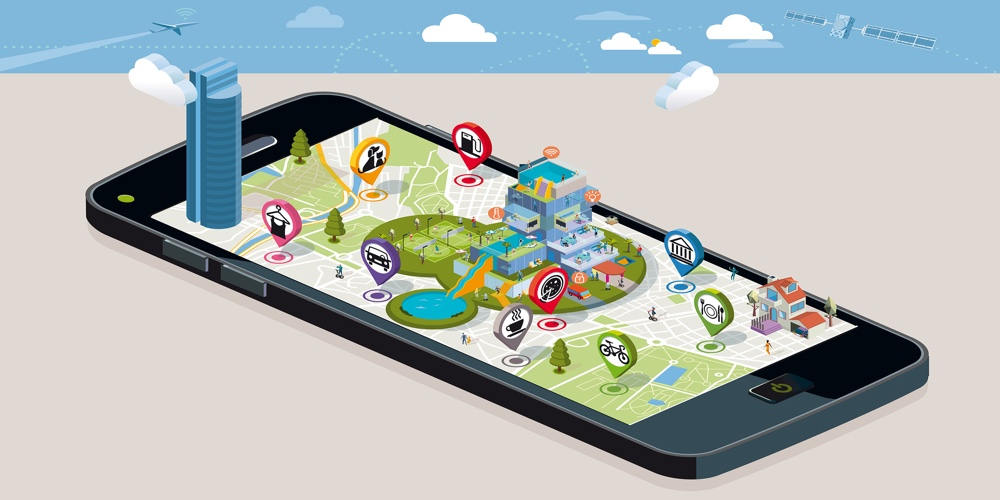
\includegraphics[width=10cm,height=4cm]{AAUgraphics/indoor}
\end{frame}
%.---------------------
% Porque Machine Learning
%.---------------------
\subsection{Porqué Machine Learning}
\begin{frame}{Introducción}{Porqué Machine Learning}
\begin{block}{Soluciones para indoor location}
\begin{center}
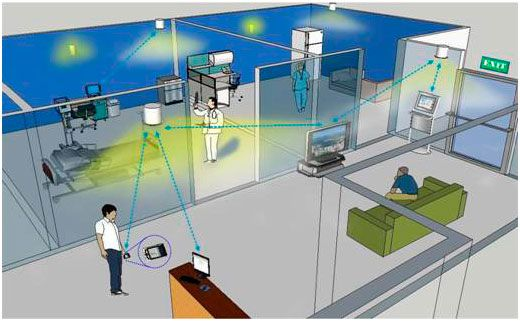
\includegraphics[scale=0.3]{AAUgraphics/ips}
\end{center}
Ecuación de Rappaport:
$$RSSI = -10 n log(d) + txPower$$
Propuesta:\\
\begin{center}
Modelar usando Machine Learning.
\end{center}
\end{block}
\end{frame}
%.---------------------
% Mapa
%.---------------------
\subsection{Definición del Problema}
\begin{frame}{Introducción}{Definición del Problema}
\begin{block}{Area Experimental}
\begin{center}
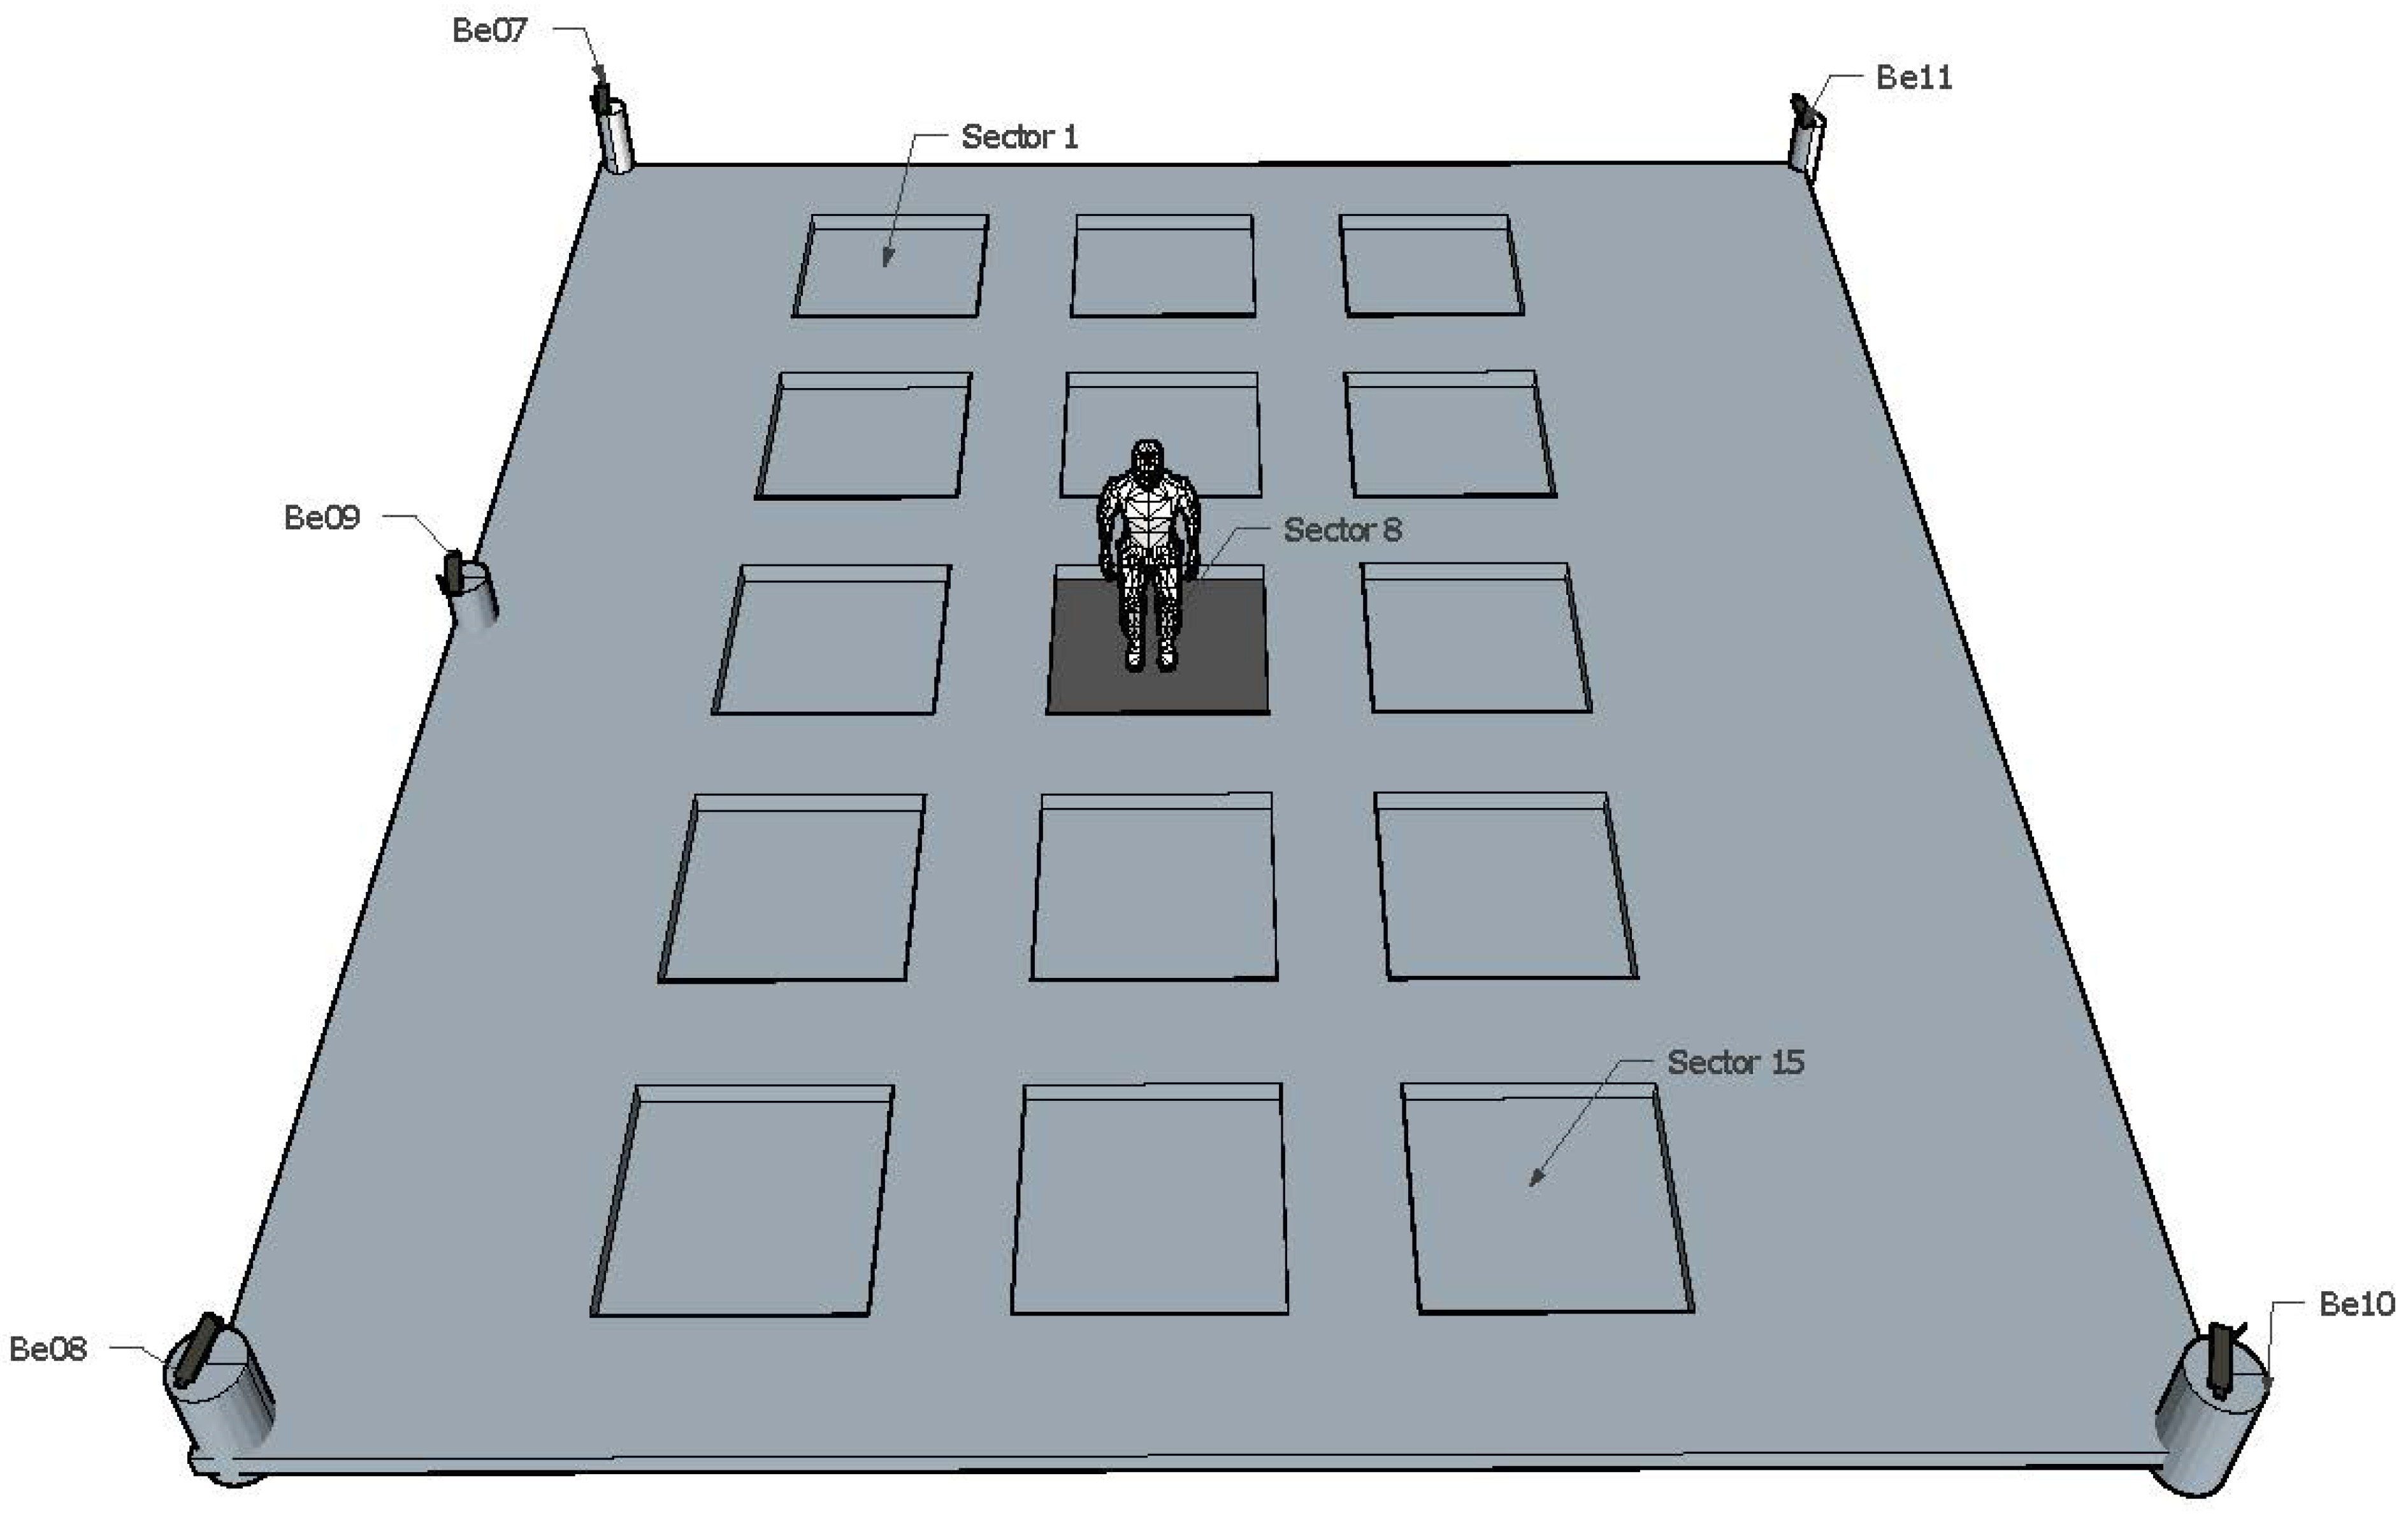
\includegraphics[scale=0.6]{AAUgraphics/sensors}
\end{center}
\end{block}
\end{frame}
%.---------------------
% Indoor Location
%.---------------------
\section{Indoor Location}
\begin{frame}{Indoor Location}{}
\begin{block}{Casos de Prueba}
El presente trabajo evalua la eficiencia para tres tipos de sucesos.\\
\begin{itemize}
	\item Caso 1:\\
	\textbf{Emisor:} Microcontroller BLE 4.0, a un único nivel de potencia.\\
	\textbf{Receptor:} Raspberry Pi con antena BLE 4.0.
	
	\item Caso 2:\\
	\textbf{Emisor:} Beacon BLE 4.0, a siete niveles de potencia.\\
	\textbf{Receptor:} Raspberry Pi con antena BLE 4.0.
	
	\item Caso 3:\\
	\textbf{Emisor:} Beacon BLE 4.0, a siete niveles de potencia.\\
	\textbf{Receptor:} Smartphone BLE 4.0.
\end{itemize}
\end{block}
\end{frame}
%.---------------------
% Casos de Prueba
%.---------------------
\subsection{Casos de Prueba}
\begin{frame}{Indoor Location}{Casos de Prueba}
\begin{block}{Caso 1: microController $\rightarrow$ RPI2}
\begin{multicols}{2}

\end{multicols}
\end{block}
\end{frame}

\begin{frame}{Indoor Location}{Casos de Prueba}
\begin{block}{Caso 2: Beacon $\rightarrow$ RPI2}
\begin{center}

\end{center}
\end{block}
\end{frame}

\begin{frame}{Indoor Location}{Casos de Prueba}
\begin{block}{Caso 3: Beacon $\rightarrow$ Smartphone}
\begin{center}

\end{center}
\end{block}
\end{frame}
%.---------------------
% Modelos
%.---------------------
\subsection{Modelos de Aprendizaje}
\begin{frame}{Indoor Location}{Modelos de Aprendizaje}
\begin{center}
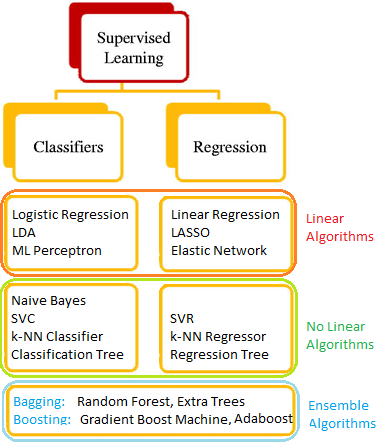
\includegraphics[scale=0.6]{AAUgraphics/map}
\end{center}
\end{frame}
%.---------------------
% Error
%.---------------------
\subsection{Accuracy y Error Medio}
\begin{frame}{Indoor Location}{Precisión y Error}
\begin{block}{Precisión}
$$Precision = nAciertos/nTest\times 100\%$$
\end{block}
\begin{block}{Error Métrico}
\begin{wrapfigure}{l}{0.3\textwidth}
    \centering
    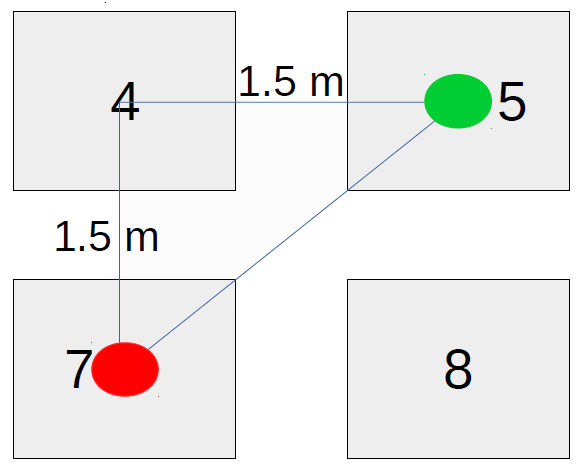
\includegraphics[width=0.3\textwidth]{AAUgraphics/espacio}
\end{wrapfigure}
$$dv = \mid p/3 - y/3\mid\times 1.5-1.0$$
$$dh= \mid p\%3 - y\%3\mid\times 1.5-1.0$$
$$d = \sqrt{dv^2 + dh^2}$$
\end{block}
\end{frame}
%.---------------------
% Resultados
%.---------------------
\section{Resultados}
%.---------------------
% Clasificación caso 1
%.---------------------
\subsection{Caso 1}
\begin{frame}{Resultados}{Caso 1: microController $\rightarrow$ RPI2}
\begin{block}{Evaluación de Clasificación}

\end{block}
\end{frame}
%.---------------------
% Regresión caso 1
%.---------------------
\begin{frame}{Resultados}{Caso 1: microController $\rightarrow$ RPI2}
\begin{block}{Evaluación de Regresión}

\end{block}
\end{frame}
%.---------------------
% tablas caso 1
%.---------------------
\begin{frame}{Resultados}{Caso 1: microController $\rightarrow$ RPI2}
\begin{multicols}{2}
\begin{block}{Clasificación}

\end{block}

\begin{block}{Regresión}

\end{block}
\end{multicols}
\end{frame}
%.---------------------
% Clasificación caso 2
%.---------------------
\subsection{Caso 2}
\begin{frame}{Resultados}{Caso 2: Beacon $\rightarrow$ RPI2}
\begin{block}{Evaluación de Clasificación}

\end{block}
\end{frame}
%.---------------------
% Regresión caso 2
%.---------------------
\begin{frame}{Resultados}{Caso 2: Beacon $\rightarrow$ RPI2}
\begin{block}{Evaluación de Regresión}

\end{block}
\end{frame}
%.---------------------
% Clasificación caso 3
%.---------------------
\subsection{Caso 3}
\begin{frame}{Resultados}{Caso 3: Beacon $\rightarrow$ Smartphone}
\begin{block}{Evaluación de Clasificación}

\end{block}
\end{frame}
%.---------------------
% Regresión caso 3
%.---------------------
\begin{frame}{Resultados}{Caso 3: Beacon $\rightarrow$ Smartphone}
\begin{block}{Evaluación de Regresión}

\end{block}
\end{frame}
%----------------------------------------------
% Conclusiones
%----------------------------------------------
\section{Conclusiones}
\begin{frame}{Conclusiones}{}
\begin{itemize}
	\item bitzer se la come doblada con triple nudo.  
	\item miguelito no me paga mis 18 lucas q me debe.  
\end{itemize}
\end{frame}
%----------------------------------------------
% Final
%----------------------------------------------
{\aauwavesbg%
\begin{frame}[plain,noframenumbering]%
  \finalpage{Gracias por su atención}
\end{frame}}

\end{document}
\grid
